\subsection{Prototipe Robot \emph{Dienen}}
\label{subsec:prototiperobotdienen}

\begin{figure} [ht]
  \centering
  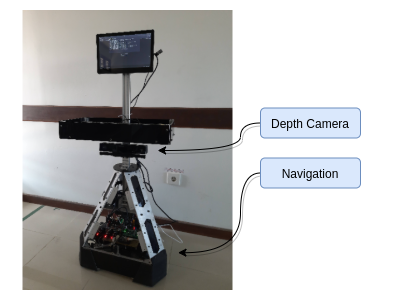
\includegraphics[scale=0.5]{gambar/komponen-prototipe-robot.png}
  \caption{Diagram komponen dari prototipe robot \emph{Dienen}.}
  \label{fig:komponenprototiperobot}
\end{figure}

Prototipe robot \emph{Dienen} ini adalah pengembangan sementara dari robot \emph{Dienen}.
Agar sesuai dengan \emph{real robot} yang diujikan,
  spesifikasi sensor dan aktuator yang digunakan oleh model robot di simulasi akan disesuaikan dengan spesifikasi komponen yang ada di prototipe robot ini.
Seperti yang terlihat pada gambar \ref{fig:komponenprototiperobot},
  prototipe robot ini saat ini baru terdiri atas komponen \emph{depth camera} dan \emph{navigation}.
Untuk komponen kamera, sebagai alternatif sementara, sebuah \emph{webcam} dapat digunakan dan dipasang ke komputer robot melalui sambungan USB.
Sedangkan untuk komponen \emph{manipulator} untuk saat ini belum bisa digunakan.

Komponen \emph{depth camera} yang digunakan di prototipe robot ini adalah Kinect V2 yang mampu menangkap citra berwarna dan citra kedalaman.
Spesifikasi kedua citra yang ditangkap tersebut memiliki perbedaan pada sisi resolusi maksimal dan \emph{field of view} (FoV),
  dimana citra berwarna bisa ditangkap hingga resolusi 1920 x 1080 dan FoV 84.1° x 53.8°,
  sedangkan citra kedalaman hanya bisa ditangkap pada resolusi 512 x 424 dan FoV 70.6° x 60°.

Komponen navigasi yang digunakan di prototipe robot ini adalah sekumpulan komponen elektronik yang digunakan di robot \emph{IRIS} \citep{cit:dikairono2020}.
Komponen tersebut terdiri atas beberapa bagian seperti motor DC, \emph{motor driver}, IMU, dsb. yang terhubung pada sebuah \emph{controller} berbasis STM32F4.
Nantinya, \emph{controller} tersebut akan terhubung dengan komputer utama dari robot yang berbasis Intel NUC melalui sambungan \emph{ethernet} dan komunikasi UDP (\emph{user datagram protocol}).

Seperti yang dijelaskan sebelumnya, kamera yang digunakan di robot adalah sebuah \emph{webcam} yang dipasang ke komputer robot melalui sambungan USB.
Kamera tersebut saat ini belum ditetapkan untuk digunakan di prototipe robot,
  namun untuk memenuhi keperluan pengujian, maka kamera tersebut dipilih untuk digunakan.
kamera yang digunakan tersebut adalah Logitech C922 yang mampu digunakan untuk menangkap citra dengan resolusi hingga 1920 x 1080.
Kamera tersebut dipilih karena kamera tersebut adalah kamera yang sama yang digunakan di robot \emph{ICHIRO} \citep{cit:muhtadin2019} yang merupakan setengah bagian asal dari robot \emph{Dienen} ini.
